\section{Architecture du code}
    Dans cette partie nous allons voir comment nous avons structuré nos programmmes, c'est un point important qui définit les performences, la robustesse et la facilité à s'adapter à de nouvelles situations de l'application produite.
    \subsection{Idée générale}
        Nous avons cherché le plus possible à utiliser les classes dès que c'était necessaire, car la \textebf{programmation orienté objet} permet une meilleure lecture du code et plus de souplesse et de facilité dans son dévelloppement.
        
        Pour la plupart des problèmes nous avons cherché à produire une \textbf{class abstraite} mère qui correspondait à l'idée générale de ce que nous voulions coder et plusieurs classe filles, plus spécifiques qui en héritait. Cette manière de proceder à l'avantage de rendre plus clair le code et de facilité l'ajout de nouvelle fonctionalité. Par exemple pour ajouter un pokemon il suffit de créer une nouvelle classe qui hérite de la classe abstraite Pokemon. 
        
        Ensuite, un autre avantage de l'orienté et de l'héritage des classes abstraites c'est de cloisonner les problèmes. En effet, quand par exemple un jeu discute avec une interface, il lui fait des requêtes (comme lui demander une action, ou appeller une animation) sans se soucier de si c'est une interface texte ou graphique.
        
        Aussi, nous avons utilisé de nombreuses property, soit pour stocker une information d'une manière différente qu'elle est utilisée, soit pour être sûr que des attributs ne sont pas modifiées en dehors de leur classe. Par exemple, pour être sûr que le pokemon courant d'un dresseurs soit un des pokemons de son dictionnaire de pokemon, self.\_\_courant stocke le nom d'un pokemon puis un property fait en sorte que self.courant soit le dictionnaire indexé par le nom stocké dans self.\_\_courant.
        
        Enfin l'orienté objet permet d'utiliser des solutions de code qui sont générales et réutilisables dans d'autres situation. Par exemple, les solution utilisant l'algorithme du minimax sont des solution générales appliquées à notre jeu.
    \subsection{Diagramme UML}
        Voici le diagramme UML de notre jeu, réalisé avec PlantText UML. Etant donné du grand nombre de classes présentent dans notre jeu, nous avons décidé de limiter le diagramme UML aux classes principales en représentant leurs classes dérivées par une seule classe Exemple. Par exemple, notre jeu comporte une classe abstraite Attaque, qui se dérive en 23 sous-classes pour les 23 différentes attaques présentent dans notre jeu. Celles-ci sont représentées dans le diagramme par la classe Exemple\_attaque.

        Dans ce diagramme, les attributs et les méthodes sont représentés respectivemement dans les parties hautes et basses des classes. Voici une légende pour mieux comprendre les signes qui peuvent apparaître devant ceux-ci.
        \bigskip
        \begin{itemize}
            \item Une classe portant la mention 'C' à côté de son nom est une classe normale
            \item Une classe portant la mention 'A' à côté de son nom, qui est écrit en italique dans ce cas, est une classe abstraite.
            \item Un rond vert non plein représente un attribut publique d'instance.
            \item Un carré rouge non plein représente un attribut privé d'instance.
            \item L'absence de signe représente un attribut de classe.
            \item Un rond vert plein représente une méthode basique.
            \item Un carré rouge plein une méthode avec une property.
            \item Une méthode soulignées représente une méthode statique.
            \item Une méthode en italique représente une méthode abstraite.

            
        
        \end{itemize}
        Remarque : pour mieux voir le diagramme, veuillez regarder directement le png(images/Diagramme\_UML)
    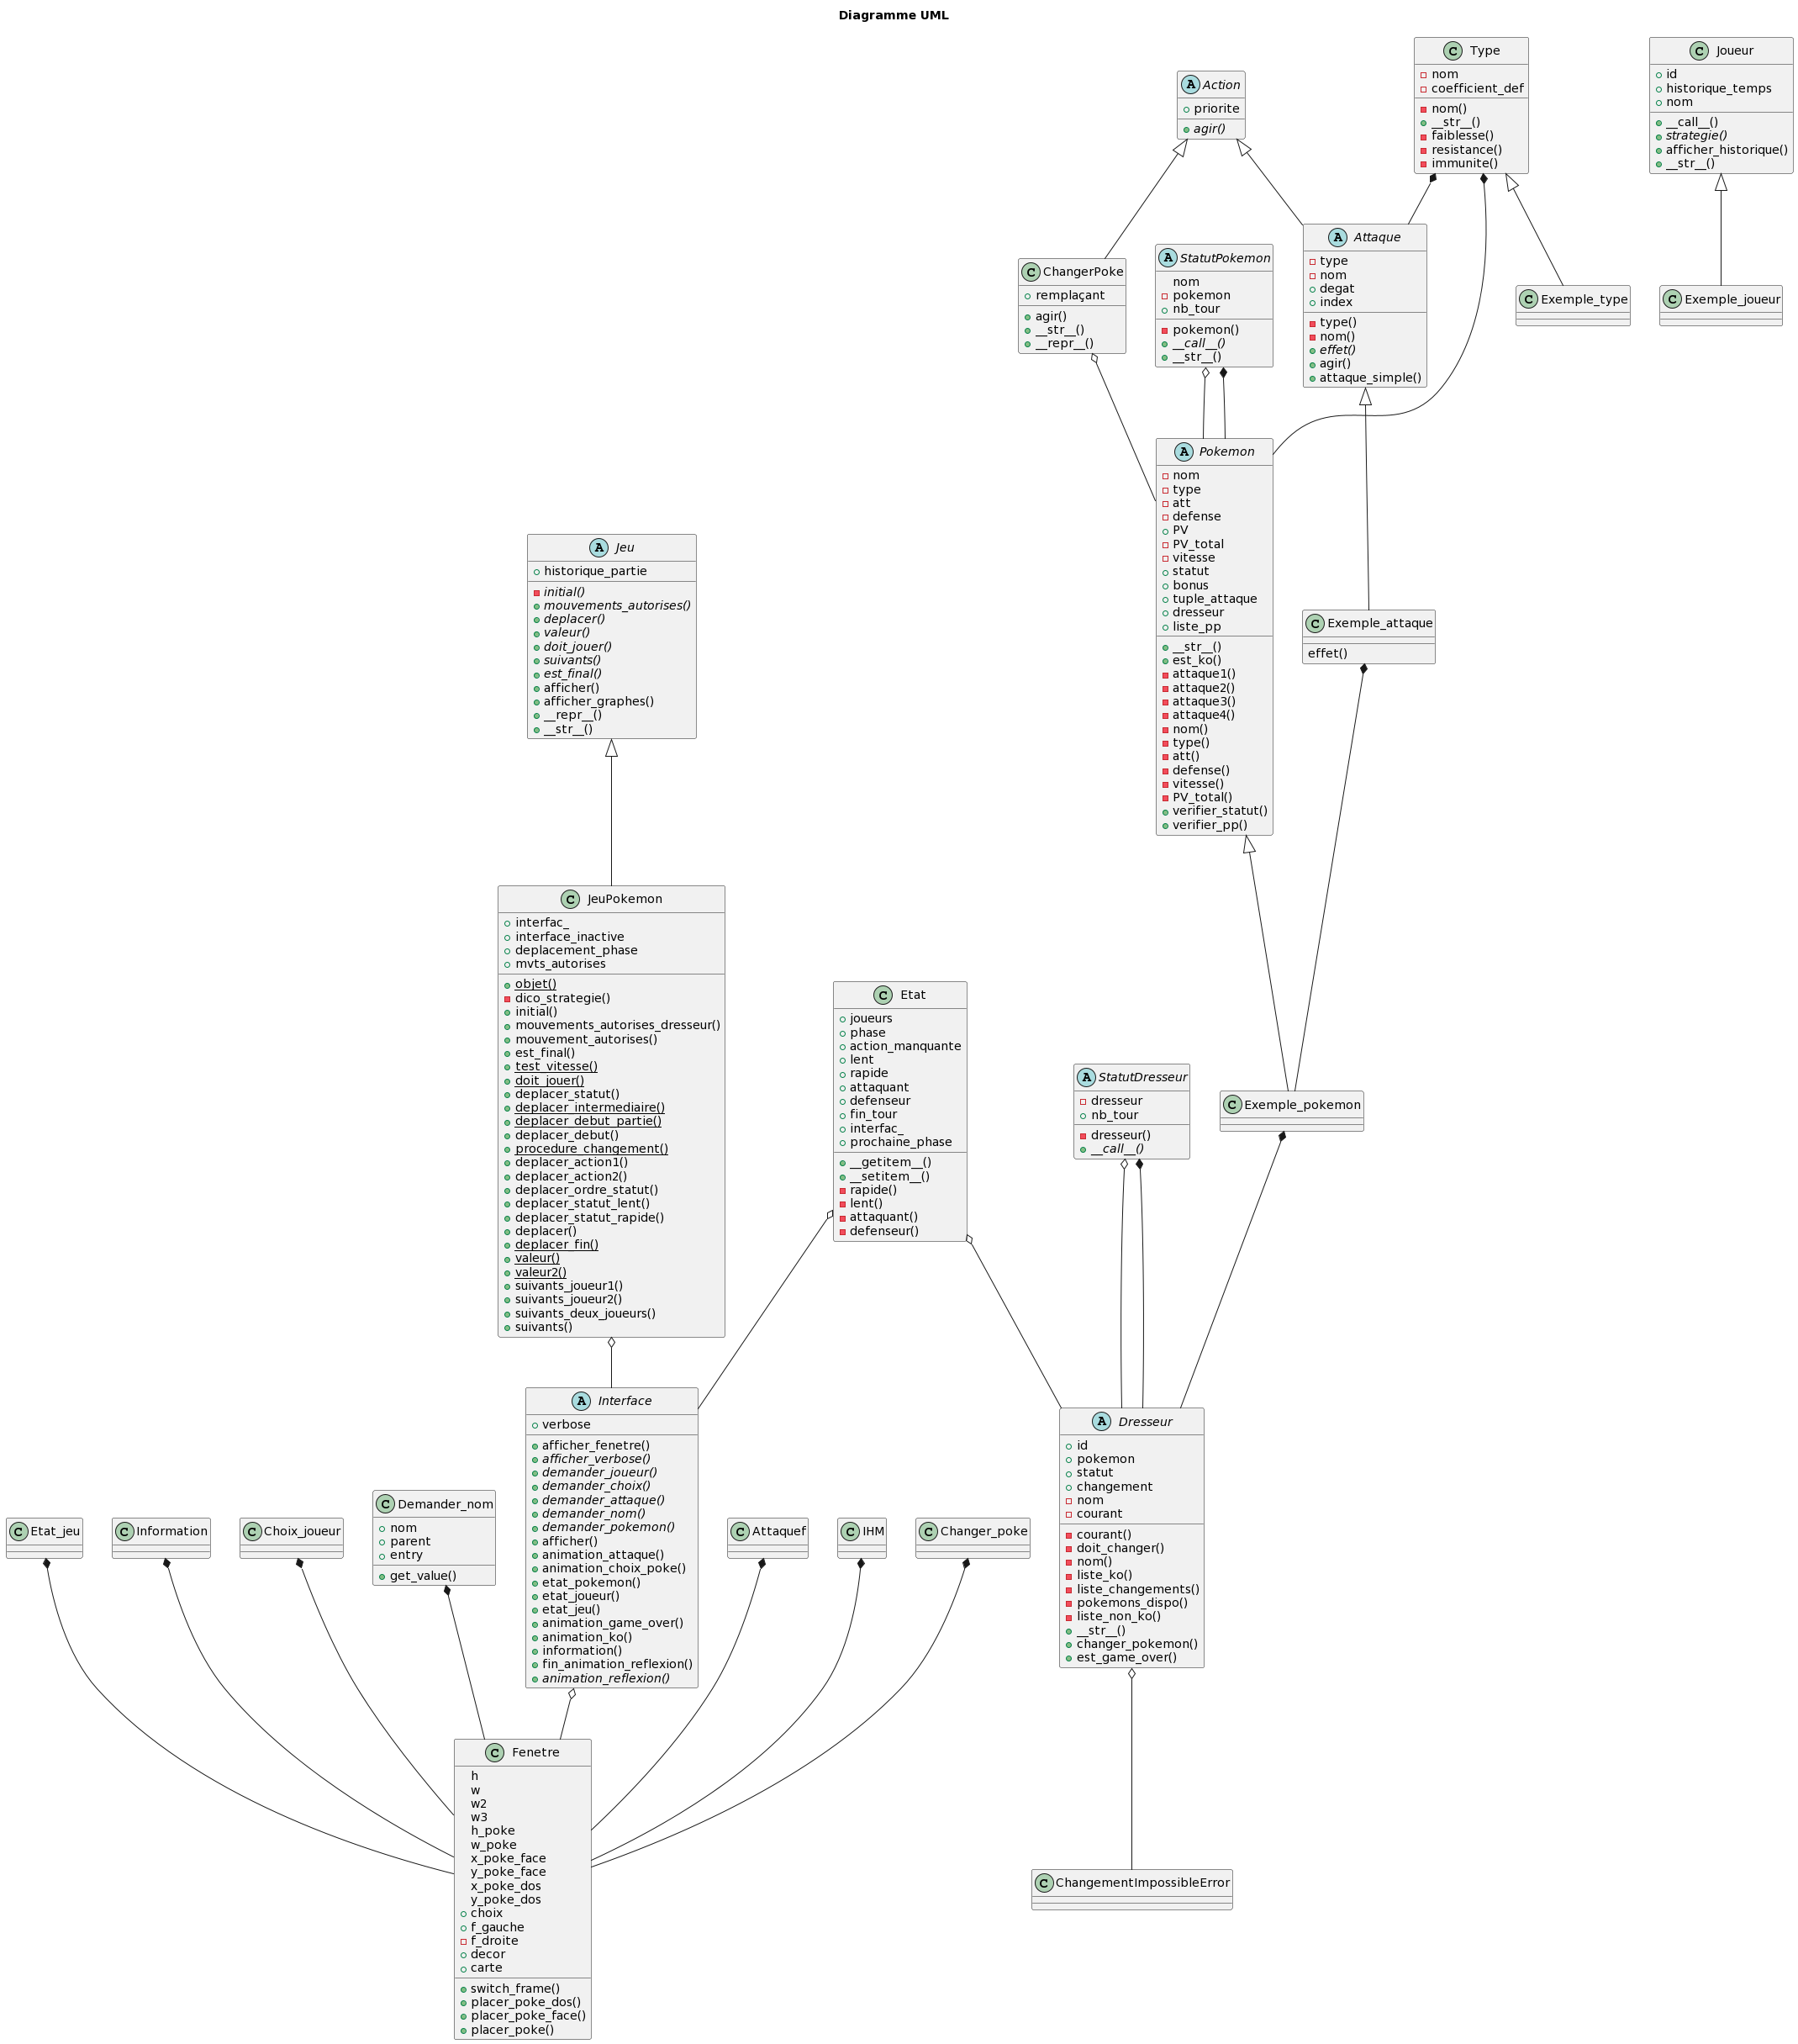
\includegraphics[width=20cm,height=20cm]{images/Diagramme_UML}
        
    \subsection{Architecture du jeu}
        Afin de pouvoir appliquer des solutions générales comme l'algorithme du minimax à notre jeu, il fallait que notre jeu soit une classe JeuPokemon qui hérite de la classe Jeu présentée dans le cours et qu'il soit lancé via joueur\_jeu.
        Pour ce qui est de la classe mère, elle a été reprise tel quel dans notre code, cependent la fonction jouer\_jeu était plus problèmatique.
        
        En effet la fonction jouer\_jeu qui nous a été présenté en cours s'appliquait a un jeu :
        \begin{itemize}
            \item à somme nulle (les interêts des joueurs sont strictement opposés).
            \item deterministe (pas d'intervention de la chance).
            \item sequentiel (l'ordre des déscisions et prédéfinit à l'avance)
            \item à information complètes (on connait ses possibilités d'action, les possibilités d'action des autres joueurs, les gains résultants de ces actions et les motivations des autres joueurs).
        \end{itemize}
        Cependent le jeu pokemon que nous vous proposons est à somme nulle, \textbf{non deterministe}, \textbf{simultané} (les joueurs décident en même temps de leur stratégie) et à information complètes.
        Nous avons donc modifié jouer jeu pour qu'elle s'applique à tout les jeux qui ont ces dernières propriétés.
        
        Aussi, nous avons transormé le while qui était dans la fonction en récursivité pour pouvoir animer le jeu avec la méthode after de tkinter mais cette modification ne change rien à ce que fait la fonction.
        Comme nous allons y faire référence dans les prochaines sections, voici la fonction joueur\_jeu:
        
        \lstinputlisting[language=Python, tabsize=1,basicstyle=\scriptsize , linerange=jouer\_jeu-end,includerangemarker=false]{code/abstract_jeu.py}
        
        \subsubsection{Jeu simultané}
            Un jeu simultané est un jeu dans lequel l'ordre de prise de déscision n'est pas prédéfinit. Selon les situation, un joueur doit prendre une descision, l'autre ou les deux en même temps. Une fois les déscision prises, un système de priorité des action permet de definir quelle action est executée en premier ou si même l'action est executée.
            Ainsi, la mèthode doit\_joueur d'un tel jeu ne renvoie pas le joueur qui jou dans un etats mais la liste des joueur qui doivent joueur.
            
            Ensuite joueur\_jeu doit demander la stratégie adoptée par chaque joueur qui doit jouer et la stocker dans deplacements qui est donc un dictionnaire qui prend comme clefs les joueurs et comme valeur les action des joueurs.
            Deplacement est ensuite fournit à deplacer pour deplacer l'etat.
        \subsubsection{Jeu non deterministe}
            Pour pouvoir prendre en compte le facteur chance, deplacer doit revoyer non pas un etat mais l'ensemble des couples des etats possibles avec leur probabilité d'apparition.
            
            Ensuite la fonction choix est utilisée pour choisir un état parmit ceux qui sont possibles.
            \lstinputlisting[language=Python, tabsize=1,basicstyle=\scriptsize , linerange=choix-end,includerangemarker=false]{code/choix.py}
        \subsubsection{Le cas particulier de pokemon}
            Pour que la classe JeuPokemon puisse respecter ce qui a été dit ci-dessus, cela a été un vrai défit de programmation.
            
            Tout d'abord un premier challenge a été de faire en sorte que la fonction deplacer s'arrête à chaque fois qu'il faut demender un choix a un des joueurs, et reprendre ensuite là où elle en était.
            Dans pokemon, un choix est demandé à chaque début de tours aux deux joueurs, puis à chaque fois qu'un pokemon est mit ko au dresseur à qui appartient le pokemon.
            \smallskip
            Ainsi, nous avons découpé le jeu en plusieurs phases, stockées dans l'etat, qui se suivent et représentent des blocs entiers sans choix posés aux joueurs. A chaque phase correspond une fonction de deplacement.
            
            De ce fait, la fonction déplacer correspond à une boucle while dans laquelle on effectue la fonction de deplacement de la phase tant que l'etat ne nous indique pas que le tour est finit.
            
            Les blocs sont les suivants :
            \begin{itemize}
                \item "debut de partie" : en tout debut de la partie, quand les dresseurs n'ont pas de poemon courant et qu'on ne peut pas faire de test de vitesse.
                \item "debut" : en debut de tour, permet de definir qui attaque en premier.
                \item "action1" : on effectue l'action du joueur qui joue en premier. 
                \item "action2" : on effectue l'action du joueur qui joue en second
                \item "ordre statut" : Si les deux joueurs ont des statuts, on definit l'ordre dans lequel ils les subiront. Si il n'y en a qu'un on les effectue directement (car pas besoin de differencier le lent et le rapide).
                \item "statut lent" : On effectue les effets de statuts du pokemon le plus lent.
                \item "statut rapide" : On efffectue les statut du joueur le plus rapide.
                \item "fin" : on verifie si on doit enlever des statuts des pokemons.
            \end{itemize}
            \paragraph{Solution au problème des interruption dans le tour :}
                A chaque fin de bloc, la phase de l'etat est mise soit à la prochaine phase soit à une phase intermédière quand un pokemon à été mit KO. L'ordre du déroulé n'est bien sur pas linéaire et ne suit pas la liste précedente. Par exemple si aucun des joueurs n'a de statut, on passe directement de "ordre statut" à "debut".
                
                Quand la phase est mise à intermédiaire, on stocke dans l'etat la prochaine phase et on signale au while que c'est la fin du tour. Ensuite le pokemon de remplacement est demandé au joueur qui a un pokemon ko et la partie reprend par le deplacement de la phase intermediaire qui effectue le changement demandé par le joueur. Puis la phase prend pour valeur la phase qui avait été stockée dans l'etat comme étant la prochaine phase et le deroulé de la partie reprend.
                
                Bien sûr, la phase qui est stockée avant une phase intermediaire comme étant la prochaine phase depend des événements dans la partie. Par exemple lors du deplacement de "action1", si c'est le joueur qui a fait l'action qui est mit KO en la faisant (par exemple si un pokemon qui a peu de PV est placé en remplacement sur des pièges de rock, il peut être mit KO), alors la prochaine phase sera "action2". Cependent si c'est le joueur qui attaque en second qui est mit KO pendent "action2", alors, la prochaine phase sera "ordre statut" car un pokemon qui est mit KO ne peut pas attaquer dans le tour.
                
                Enfin pour que la partie puisse reprendre correctement après une interruption, on est parfois amené à stocker dans l'etat des information comme l'attaque du second attaquant ou le pokemon qui doit subir les statuts lent... Ce stokage est fait dans l'etat qui est donc une instence de la classe Etat. La classe Etat possède de nombreux attributs dont ces informations intermediaires, la phase, les dresseurs... (voir abstract\_jeu.py)
            \smallskip
            \paragraph{Deplacement de tout les Etats possibles :}
                Le déroulé présenté dans le paragraphe précédent correspond à la fonction deplacer telle qu'elle était avant qu'on ne prenne en compte l'aléatoire.
                
                Ainsi deux changement majeur on été fait pour prendre en compte les branches liées à la chance : 
                \begin{itemize}
                    \item Toutes les action renvoient des couples d'etat possibles avec la probabilité associée, ainsi, toute les fonctions de deplacement renvoient elles aussi le même type de couple.
                \end{itemize} La fonction deplacer travaille avec des listes qui stockent tout les etats possible qui ne sont pas encore finit, et a chaque tour du while, elle parcours la liste pour deplacer la phase suivante de tout ces etats.  A chaque fois qu'un etat est déplacé, ce qui est récupéré est une liste d'etats possible liés au deplacement de cet etat particulier, la probabilite de tout les etats de cette liste est donc multipliée par la probabilite de l'etat dont ils sont issus.
                
                A chaque fois qu'un etat est finit, il est stocké avec sa probabilité dans la liste finale, sinon il est stoké avec sa probabilité dans une liste des etats qui restent à deplacer. La boucle while s'arrête quand il ne reste plus d'etats possibles qui ne sont pas finits.
                
        \subsubsection{Les fonctions suivants}
            Pour les jeu simultanés il y a une petite subtilité par rapport aux etats suivant, c'est que si l'autre joueur doit joueur dans l'etat suivant, il faut présicer quelle action il fait pour réelement, c'est ce qui a été fait dans notre jeu. Ainsi, il ya a deux fonction suivant qui ont principalement été utilisée : suivants\_joueur1 et suivants\_joueur2. On leur fournit deux informations : l'etat et si l'autre joueur joue avec dans ce cas là, son action. La fonction renvoie l'ensemble des triplet action du joueur 1, action du joueur 2, liste des etats possibles avec leur probabilité, sachant que les action de l'autre joueur seront donc soit toutes les même si il joue soit None si il ne joue pas
            
            Voici le code :
            
            \lstinputlisting[language=Python, tabsize=1,basicstyle=\scriptsize , linerange=suivant-end,includerangemarker=false]{code/jeu.py}